\section{Evaluation Setup}
    \begin{figure}
        \centering
        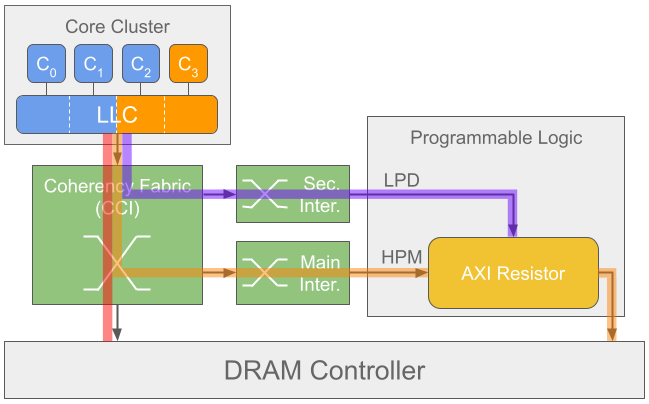
\includegraphics[scale=0.35]{images/Evaluation_setup.png}
        \caption{}
        \label{}
    \end{figure}
    jailhouse \cite{jailhouse}, ARM cortex-a53 \cite{ARM-cortex-A53}, Xilinx ZCU102 \cite{Xilinx-ULTRASCALE-TRM}, SD-VBS \cite{SD-VBS}, PLIM \cite{PLIM20}

    \subsection{Processing System Organization}
        \begin{itemize}
            \item Jailhouse used to partition the cache (via cache coloring), ensuring that the results will not be stained with inter-core evictions. Furthermore, it isolates the Software stack, ensuring that the observed delays do not come from the operating systems safety mechanisms.
            \item In the following experiments, only two virtual machines are used. One referred to as the \emph{victim} and the other referred to as the \emph{polluter}. The \emph{victim} virtual machine is a full fledge Linux system tasked to run a givan payload. The \emph{victim} VM features three cores and has half of the LLC allocated as private cache. The \emph{polluter} VM is a lightweight baremetal application in charge of emitting sequential read transactions toward the desired target. The latter runs on one core. We enforce that only one transaction at a time is sent to the target by (1) inserting a \emph{Data Synchronisation Barrier} instruction (or \texttt{DSB}) after each read and (2) having one cache partition for the code located in main memory and another cache partition for to store the read transactions mapping the target memory.
        \end{itemize}

    \subsection{Attacker - Reading Memory Bomb}
    \subsection{AXI-Resistor IP}
